\documentclass{article}
\usepackage{amsmath}
\usepackage{graphicx}
\usepackage[a4paper, margin=1in]{geometry}
\usepackage{pgfplots}
\pgfplotsset{compat=1.17}
\usepackage{afterpage}
\usepackage{float}
\usepackage{hyperref}
\usepackage{subcaption}
\graphicspath{{assets/}}

\title{Crypto Monitor on a Real Time Embedded System}
\author{Epameinondas Bakoulas}
\date{July 2025}

\begin{document}

\maketitle

\section{Objective}
Our goal in this project is to implement a crypto monitor that will run on a raspberry-pi continuously.
It will collect data via a websocket for a total of 8 different symbols, perform some calculations for
each symbol and save the results on .txt files.

Later on, we will expand on this idea by performing other calculations out of the scope of this project,
in order to better predict the market and make better decisions on when to buy or sell.

\section{Analysis}

\subsection{Overview}
Our analysis will be performed on 8 different cryptocurrency symbols, which are
BTC-USDT, ADA-USDT, ETH-USDT, DOGE-USDT, XRP-USDT, SOL-USDT, LTC-USDT, BNB-USDT, and 
we will use the the OKX Websocket public channel to collect the exchange data.

We're going to perform a total of 2 calculations for each symbol.
\begin{itemize}
    \item Calculate the moving average price and volume of the symbol for the last 15 minutes.
    \item Calculate the pearson correlation with all other symbols (and itself).
\end{itemize}

These calculations are going to be performed every minute and the results will be saved on a .txt file.
We are using a total of 5 threads, one for the websocket connection, one for the main function that checks if the connection
is active, and the other 3 are for the scheduler, moving average and pearson correlation calculations.

\subsection{Collecting data and fault tolerance}
We will use the library \texttt{libwebsockets} to connect to the OKX websocket public channel and collect the exchange data.

In order to ensure that the connection can be re-established in case of a disconnection, we will implement a reconnection 
mechanism that will attempt to reconnect every 5 seconds until successful. This is done in 2 parts. First, we
check if the connection is lost, and then we check if the subscriptions to the symbols are active. If not, we assume 
that the connection isn't established and we attempt to reconnect.

If the connection is lost, the moving average and pearson correlation calculations are still performed,
using only the latest valid values.


\subsection{Storing measurements}
The measurements (exchanges) that arrive via the websocket will be saved in 2 places:
\begin{itemize}
    \item In-memory for quick retrieval and calculations (last 15 minutes only), on a double-ended queue.
    \item In .txt files for long-term storage and analysis, separate for each symbol.
\end{itemize}

\subsection{Scheduler}
The calculations should be performed every minute on the minute mark. In order to achieve this, we will spawn
a thread called \texttt{threadScheduler} that will run continuously and signal the threads \texttt{threadAverage}
and \texttt{threadPearson} on the minute mark to perform the calculations.

In order to signal the threads to perform the calculations, we will use a combination of mutexes and condition variables, as
well as use a boolean called \texttt{workReady}. When the time comes, the \texttt{threadScheduler} will lock the mutex, 
set \texttt{workReady} to true, and notify the condition variable. This way, we can safely signal the other threads 
to perform the calculations.

The scheduler is also responsible for cleaning up the old in-memory data right before we perform the calculations.


\subsection{Moving Average price calculation}
We're going to calculate the 15-minute moving average of both the price and volume using the following formula:

\begin{equation*}
\text{MA} = \frac{1}{15} \sum_{i=1}^{15} p_{\text{close},i}
\end{equation*}

where $p_{\text{close},i}$ represents the closing price/volume at minute $i$ within the last 15-minute window.


\subsection{Pearson Correlation calculation}
In order to calculate the pearson correlation between a symbol and all other symbols we will do the following:

\begin{enumerate}
    \item Get the latest 8 moving averages of the 1st symbol
    \item Create a sliding 8-element window of the moving averages of the 2nd symbol, using the last hour values
    \item Calculate the pearson correlations ($60-8+1=53$ total) between the 1st symbol and the 2nd symbol
    \item Repeat this process by changing the 2nd symbol
    \item Find the maximum correlation value and its index
    \item Save the results in a .txt file
\end{enumerate}

In case the 1st and 2nd symbols are the same, the sliding window will stop at the 9th latest MA.

The formula for the pearson correlation is:
\begin{equation*}
r = \frac{\sum_{i=1}^{n} (x_i - \bar{x})(y_i - \bar{y})}{\sqrt{\sum_{i=1}^{n} (x_i - \bar{x})^2 \cdot \sum_{i=1}^{n} (y_i - \bar{y})^2}}
\end{equation*}

where $x_i$ and $y_i$ are the moving averages of the 1st and 2nd symbols respectively, $\bar{x}$ and $\bar{y}$ are their means, and $n$ is the number of elements in the sliding window (8).

\section{Results}

\subsection{Delays for moving average calculations}
The results are produced on a \textbf{Raspberry Pi Zero 2W} with a 1GHz quad-core CPU and 512MB of RAM.
Figures \ref{alg:delay-ma-btc} and \ref{alg:delay-ma-bnb} show the distribution of the calculation delays 
for the moving average using box plots, for the symbols \texttt{BTC-USDT} (first symbol out of the 8) 
and \texttt{BNB-USDT} (last symbol, highest delays). The delays are measured in milliseconds.

We can clearly see that the delays are generally below 20ms, and we never calculate the moving averages before
the minute mark (i.e. the delay is always positive). There are some edge cases where the delay reaches above 1000ms,
but this is very rare.

\begin{figure}[H]
    \centering
    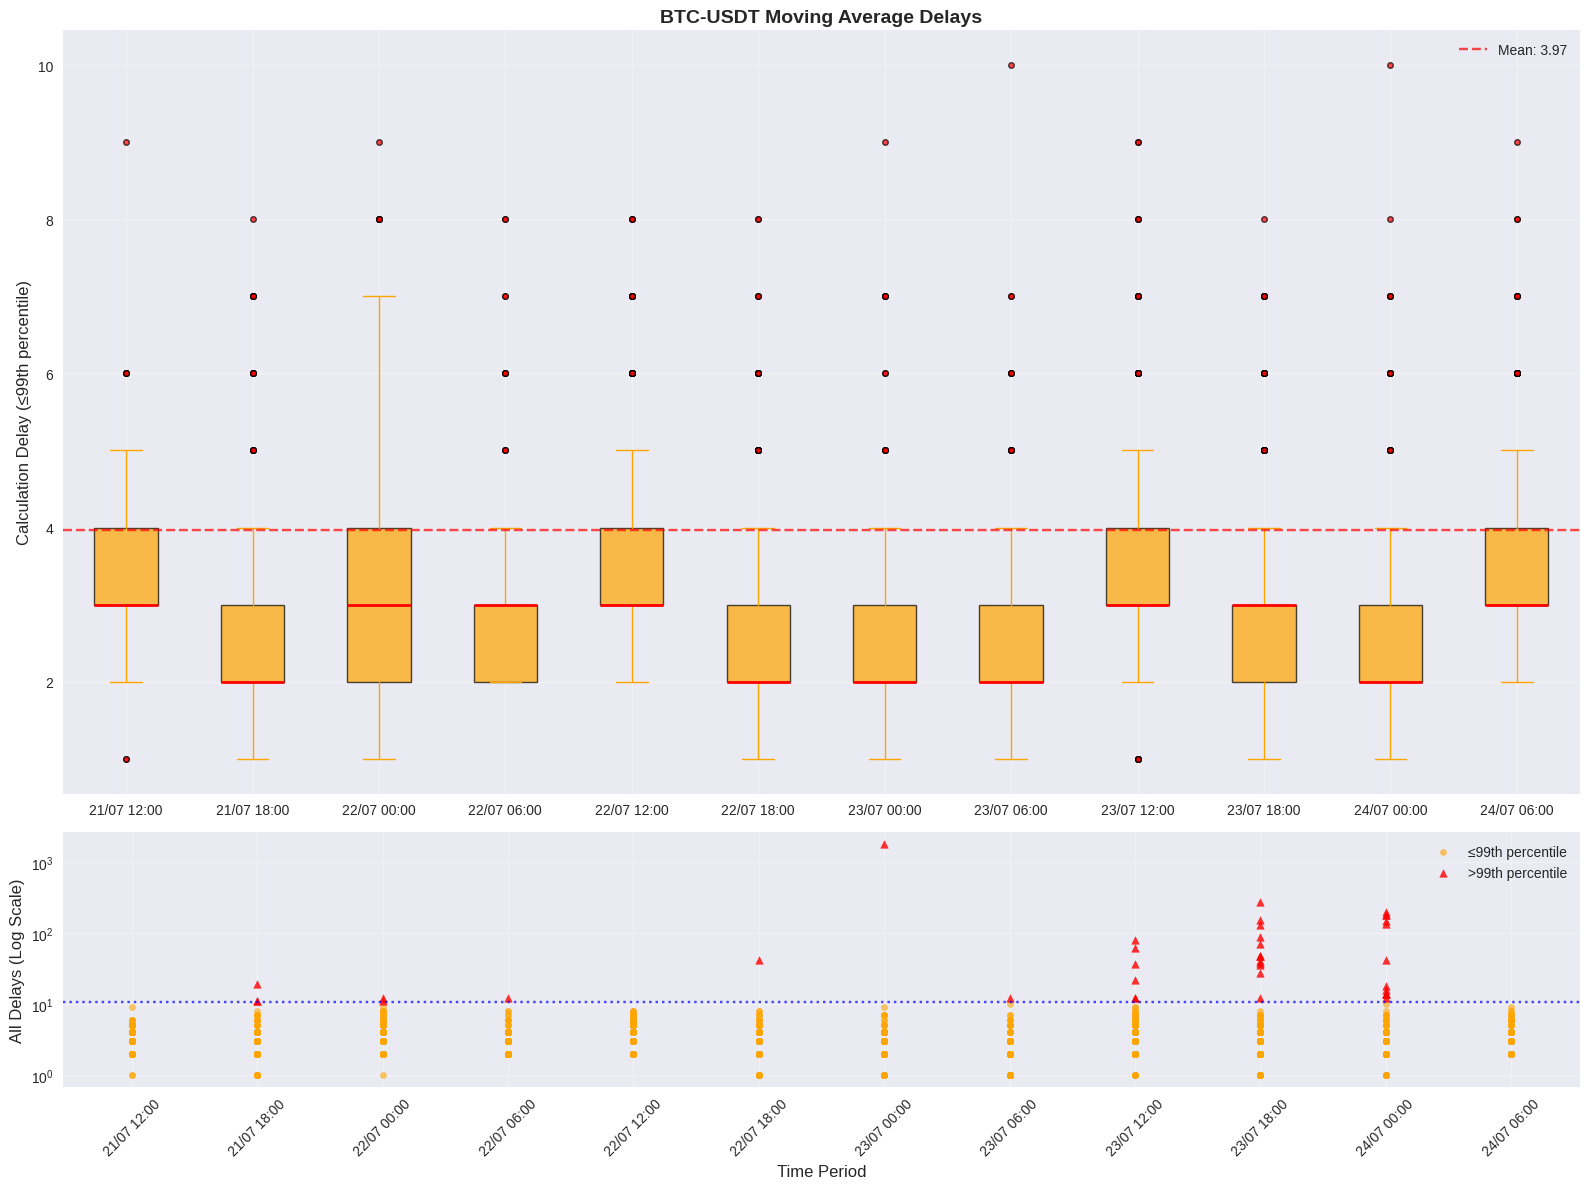
\includegraphics[width=0.9\textwidth]{boxplot-MA-BTC.png}
    \caption{Moving average calculation delays for BTC-USDT (in ms)}
    \label{alg:delay-ma-btc}
\end{figure}

\begin{figure}[H]
    \centering
    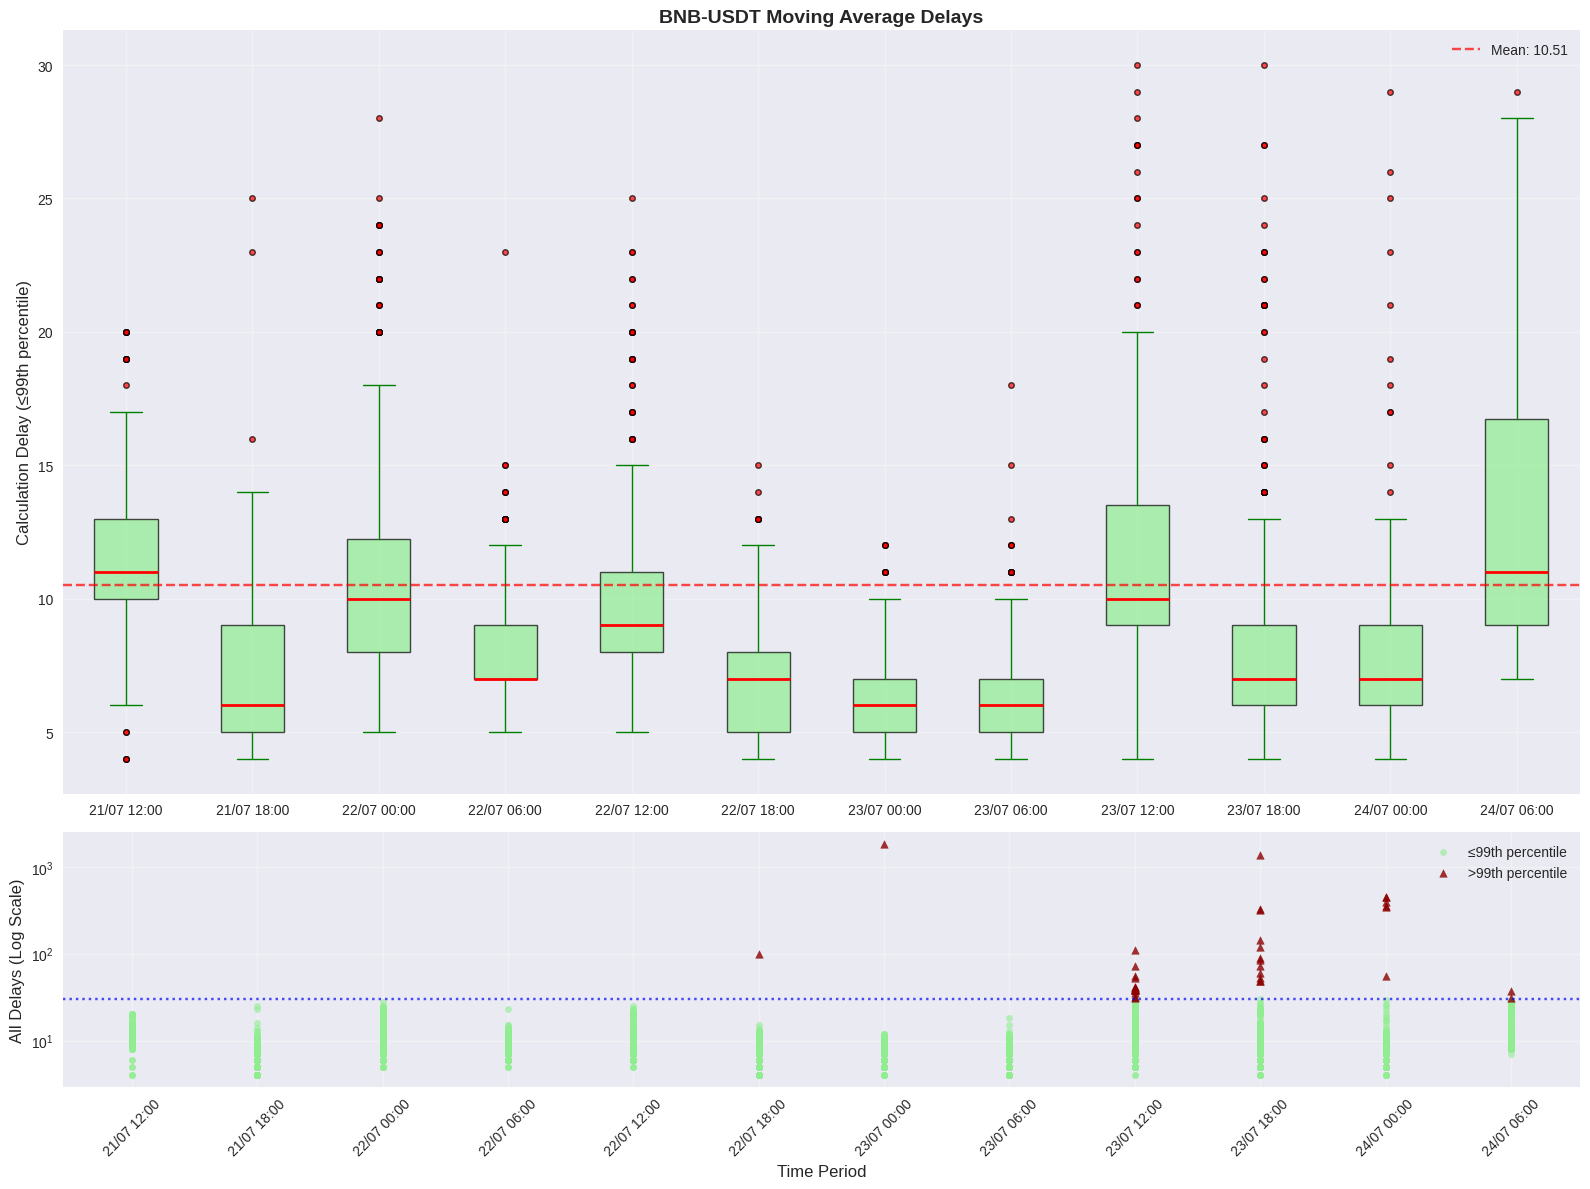
\includegraphics[width=0.9\textwidth]{boxplot-MA-BNB.png}
    \caption{Moving average calculation delays for BNB-USDT (in ms)}
    \label{alg:delay-ma-bnb}
\end{figure}

\subsection{Delays for pearson correlation calculations}
Similarly, figures \ref{alg:delay-pc-btc} and \ref{alg:delay-pc-bnb} show the distribution of the calculation delays 
for the pearson correlation.
The delays are generally below 40ms, while on the edge cases we reach above 1000ms.

\begin{figure}[H]
    \centering
    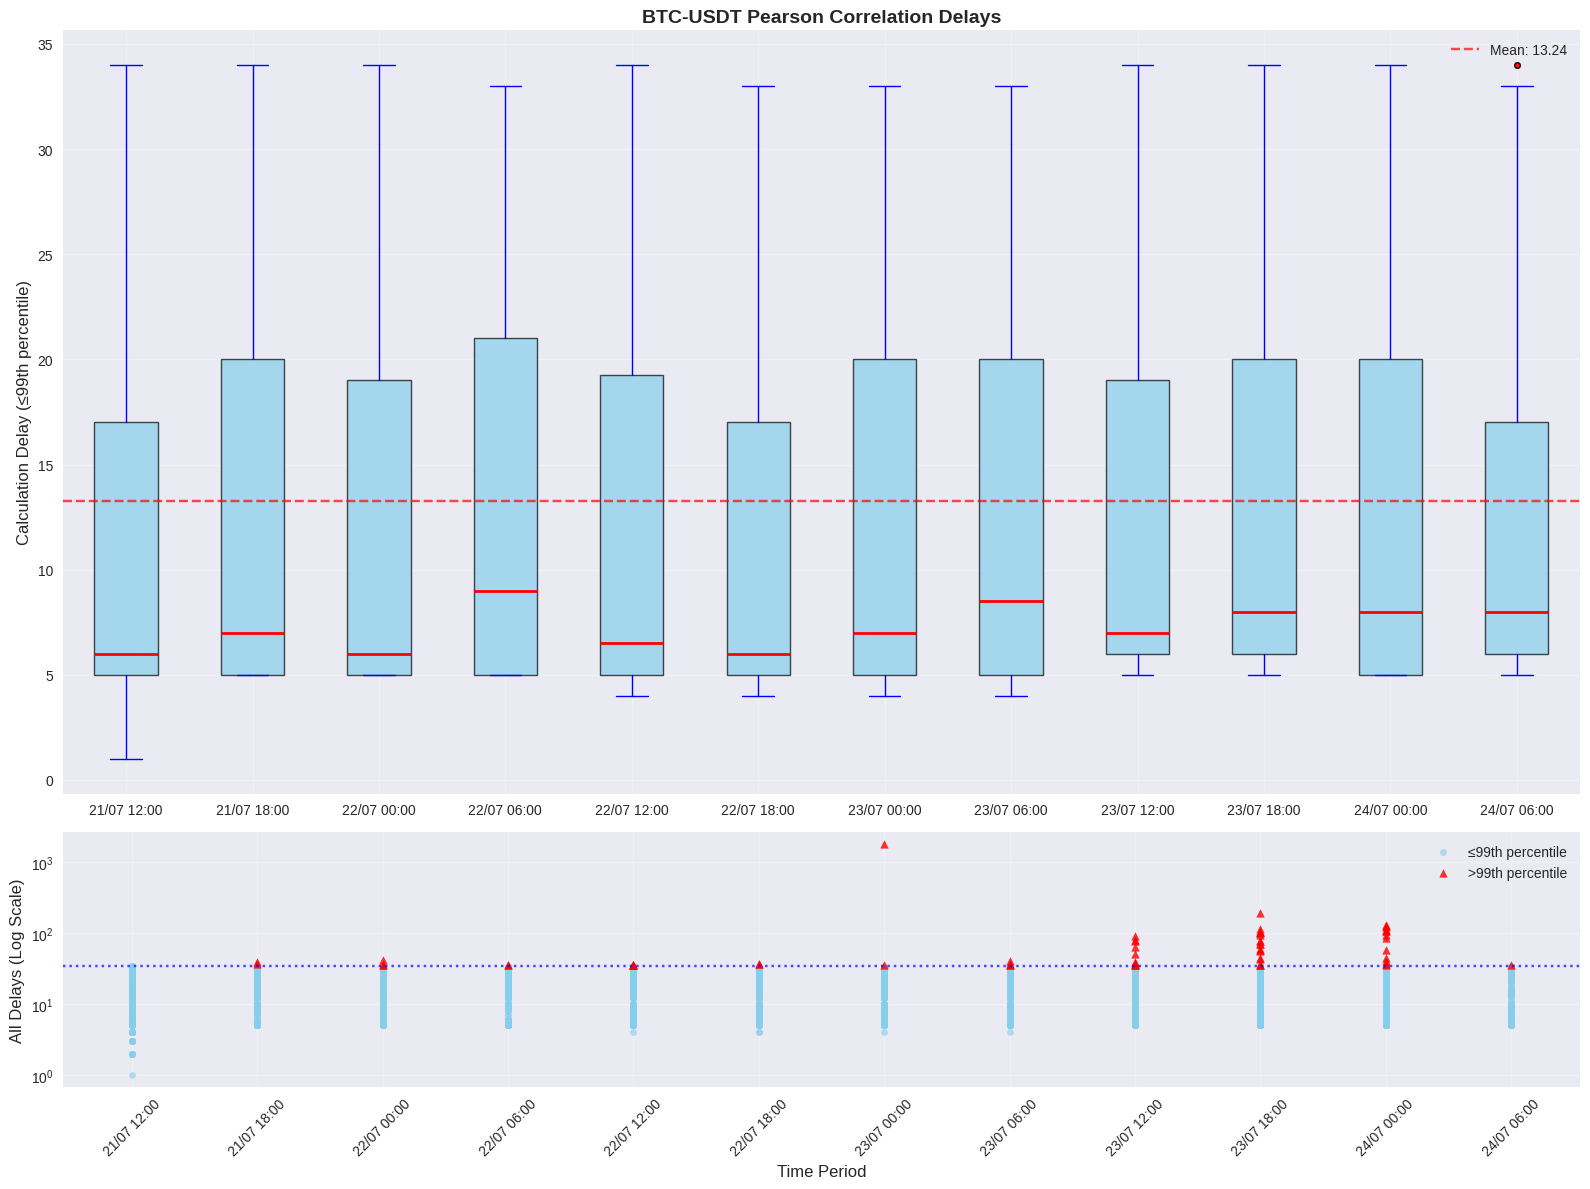
\includegraphics[width=0.85\textwidth]{boxplot-PC-BTC.png}
    \caption{Pearson correlation calculation delays for BTC-USDT (in ms)}
    \label{alg:delay-pc-btc}
\end{figure}

\begin{figure}[H]
    \centering
    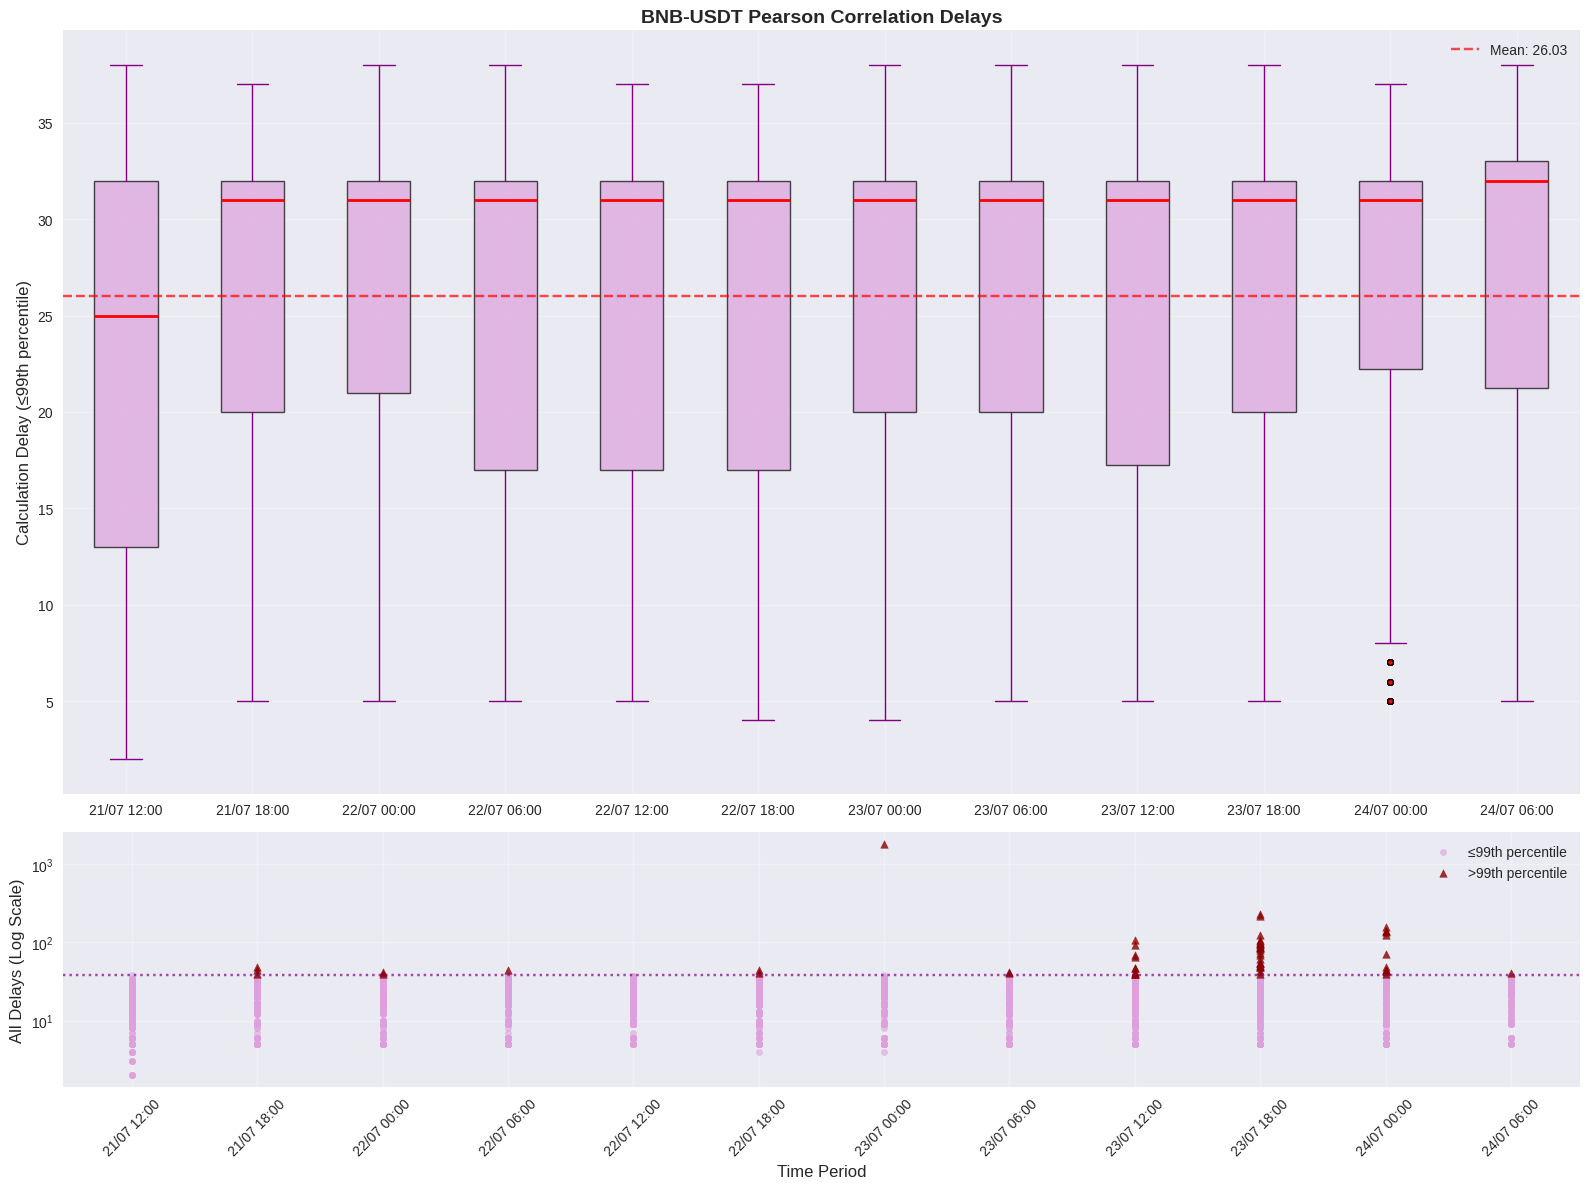
\includegraphics[width=0.85\textwidth]{boxplot-PC-BNB.png}
    \caption{Pearson correlation calculation delays for BNB-USDT (in ms)}
    \label{alg:delay-pc-bnb}
\end{figure}

\subsection{CPU Utilization}
Lastly, figure \ref{alg:delay-cpu} shows the distribution of the CPU idle percentage throughout the calculations.
The CPU idle percentage is generally above 96\%, while on the edge cases it can drop to 90\%. Generally,
the CPU is not heavily utilized, which is a good thing in case we have a limited supply of power.

\begin{figure}[H]
    \centering
    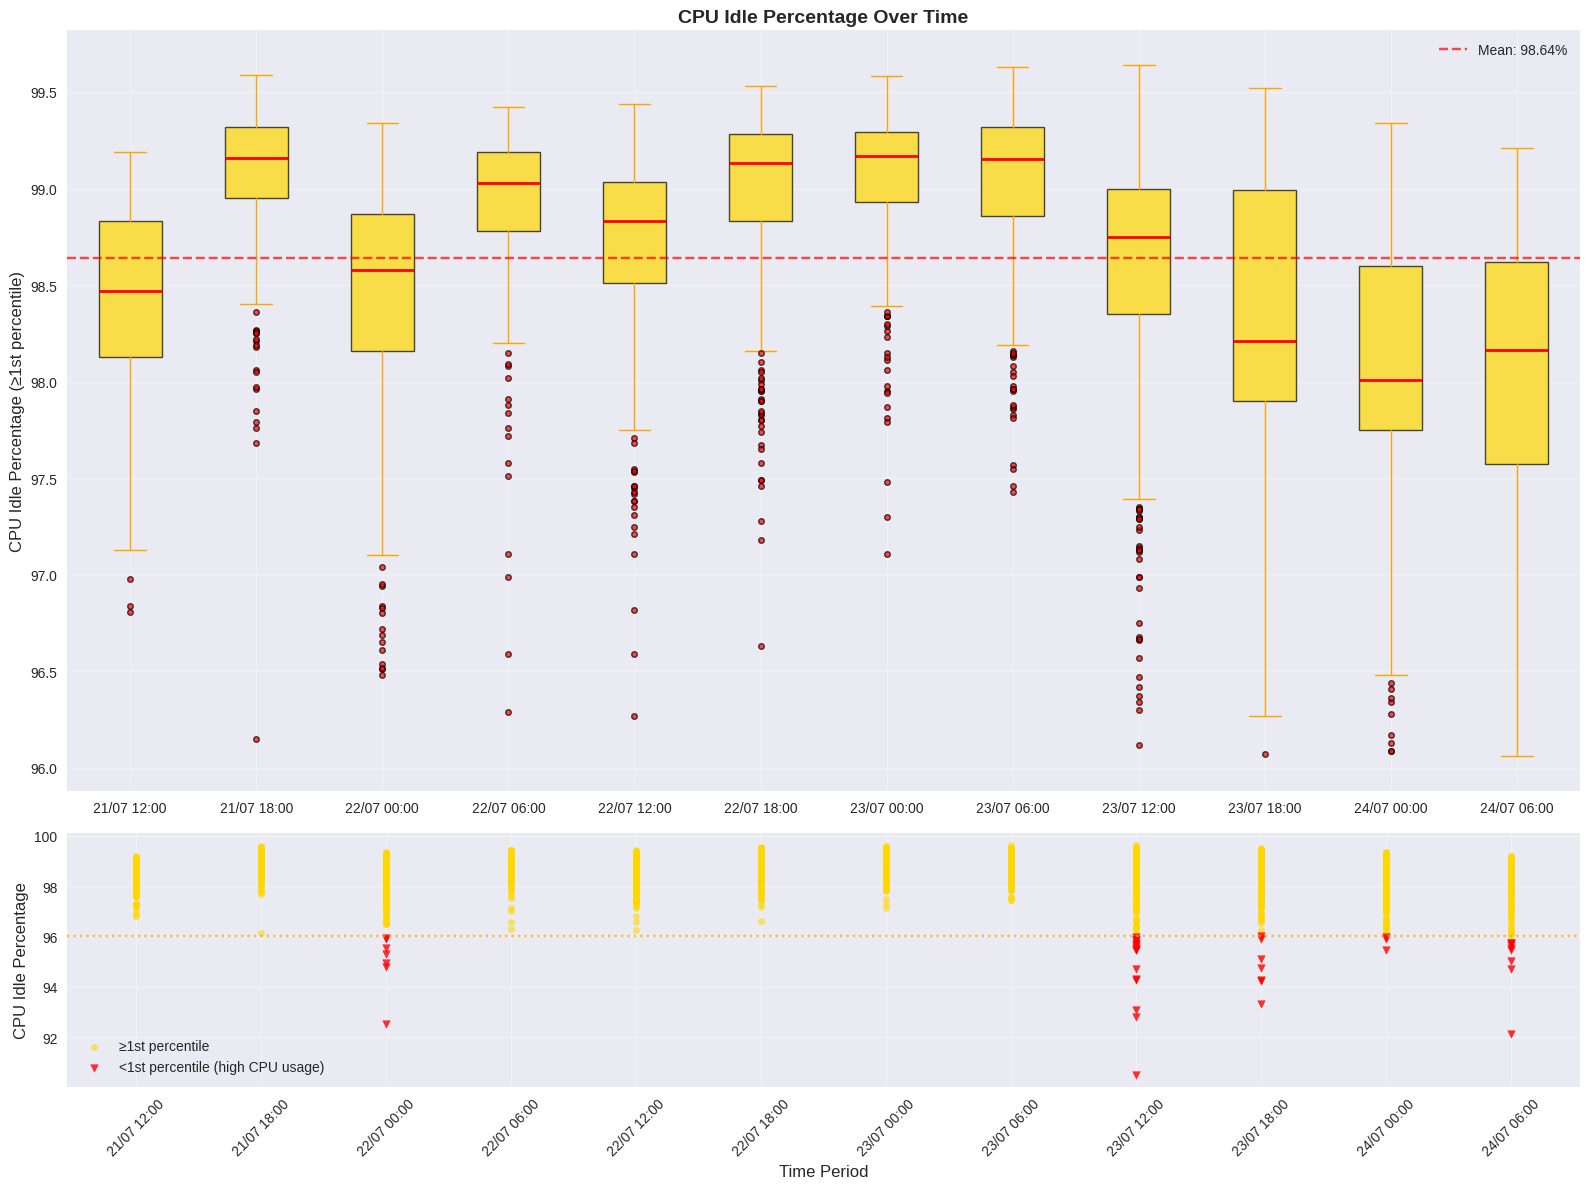
\includegraphics[width=0.9\textwidth]{boxplot-CPU.png}
    \caption{CPU idle percentage}
    \label{alg:delay-cpu}
\end{figure}


\section{Predicting the market}
On this section, we are going to make some modifications/additions to the code in order to predict the market
bettter. The steps we're going to follow are the following:

\begin{enumerate}
    \item Instead of calculating only the \texttt{MA} (or \texttt{Simple Moving Average}, \texttt{SMA}) of the price,\
    we will also calculate the \texttt{EMA} (\texttt{Exponential Moving Average}) of the price.
    \item We will also calculate the \texttt{MACD} (\texttt{Moving Average Convergence Divergence}) of the price\
    as well as the \texttt{signal line} of the \texttt{MACD} and the \texttt{Distance} between the \texttt{MACD}\
    and the \texttt{signal line}.
    \item We'll use the above indicators to make predictions on when to buy/sell stocks.
    \item Lastly, we will deploy a web server and display all of these lines on a web browser as well as the\
    timestamps on when to buy/sell stocks.
\end{enumerate}

These metrics are of high importance if we want to make better financial decisions.

\subsection{Exponential Moving Average (EMA)}
The \texttt{EMA} is a type of moving average that places a greater weight and significance on the most recent data points.
This means that it reacts more significantly to recent price changes compared to the \texttt{SMA}, which 
treats all data points equally.

We will calculate two different \texttt{EMA} values, one will be the \texttt{Short term EMA} (12 hours),
and the other will be the \texttt{Long term EMA} (26 hours). The formula for the \texttt{EMA} is as follows:
\begin{equation*}
\text{EMA} = \begin{cases}
P_{\text{current}} & \text{if } \text{EMA}_{\text{previous}} = 0 \\
(P_{\text{current}} - \text{EMA}_{\text{previous}}) \cdot \alpha + \text{EMA}_{\text{previous}} & \text{otherwise}
\end{cases}
\end{equation*}

where:
\begin{align*}
n &= 12 \text{ or } 26 \\
\alpha &= \frac{2}{n + 1} \\
P_{\text{current}} &= \text{current price}
\end{align*}

This formula assumes that we're calculating the \texttt{EMA} every hour, but since we're going to be calculating it
every minute some modifications are needed (i.e. \texttt{n} will be much larger and alpha will be much smaller).
The results will be the same. By using large windows (12/26 hours, instead of minutes), we can achieve better results
with more sporadic buy/sell signals.

For comparison, we change the window for the \texttt{SMA} to 15 hours (results displayed on the frontend).

\subsection{EMA Strategy}
The strategy on when to buy/sell is as follows, when there's a crossover between the two EMAs:
\begin{itemize}
    \item When the short-term EMA crosses above the long-term EMA, this indicates a bullish signal and we should buy
    \item When the short-term EMA crosses below the long-term EMA, this indicates a bearish signal and we should sell
\end{itemize}

\subsection{MACD Indicator}
The \texttt{MACD} is a trend-following momentum indicator that shows the relationship between two EMAs.
In order to calculate it, all we have to do is subtract the long-term EMA from the short-term EMA:
\begin{equation*}
\text{MACD} = \text{EMA}_{\text{short}} - \text{EMA}_{\text{long}}
\end{equation*}

\subsection{Signal Line}
The \texttt{Signal Line} is a 9-hour EMA of the \texttt{MACD}. It is used to generate buy/sell signals based on the MACD line.

\subsection{Distance between MACD and Signal Line}
The \texttt{Distance} between the \texttt{MACD} and the \texttt{Signal Line} is calculated as follows:
\begin{equation*}
\text{Distance} = \text{MACD} - \text{Signal Line}
\end{equation*}

\subsection{MACD, Signal and Distance Strategy}
The strategy on when to buy/sell is as follows, when there's a crossover between the MACD and the Signal Line:
\begin{itemize}
    \item When the MACD crosses above the Signal Line, this indicates a bullish signal and we should buy
    \item When the MACD crosses below the Signal Line, this indicates a bearish signal and we should sell
\end{itemize}

This is a very strong indicator, and it is used by many traders to make decisions on when to buy/sell stocks.
In our case, we used the MACD(12,26,9) which is used by many traders and produces good results.

\section{Web Server}
In order to display the results, we will attach a REST web server to the \texttt{C++} application.
This web server will have some endpoints (for example \texttt{/ema?window=100\&symbol=BTC-USDT})
that will server the data. In order to safely serve this data (without exposing home IP addresses),
the server is hosted on a VPS by DigitalOcean.

The frontend is created using \texttt{React} with the help of \texttt{Vite, Tailwind} and \texttt{Shadcn UI}.
Utilizing Cloudflare's Workers (serverless platform), we can cheaply and securely host the frontend.

\begin{figure}[H]
    \centering
    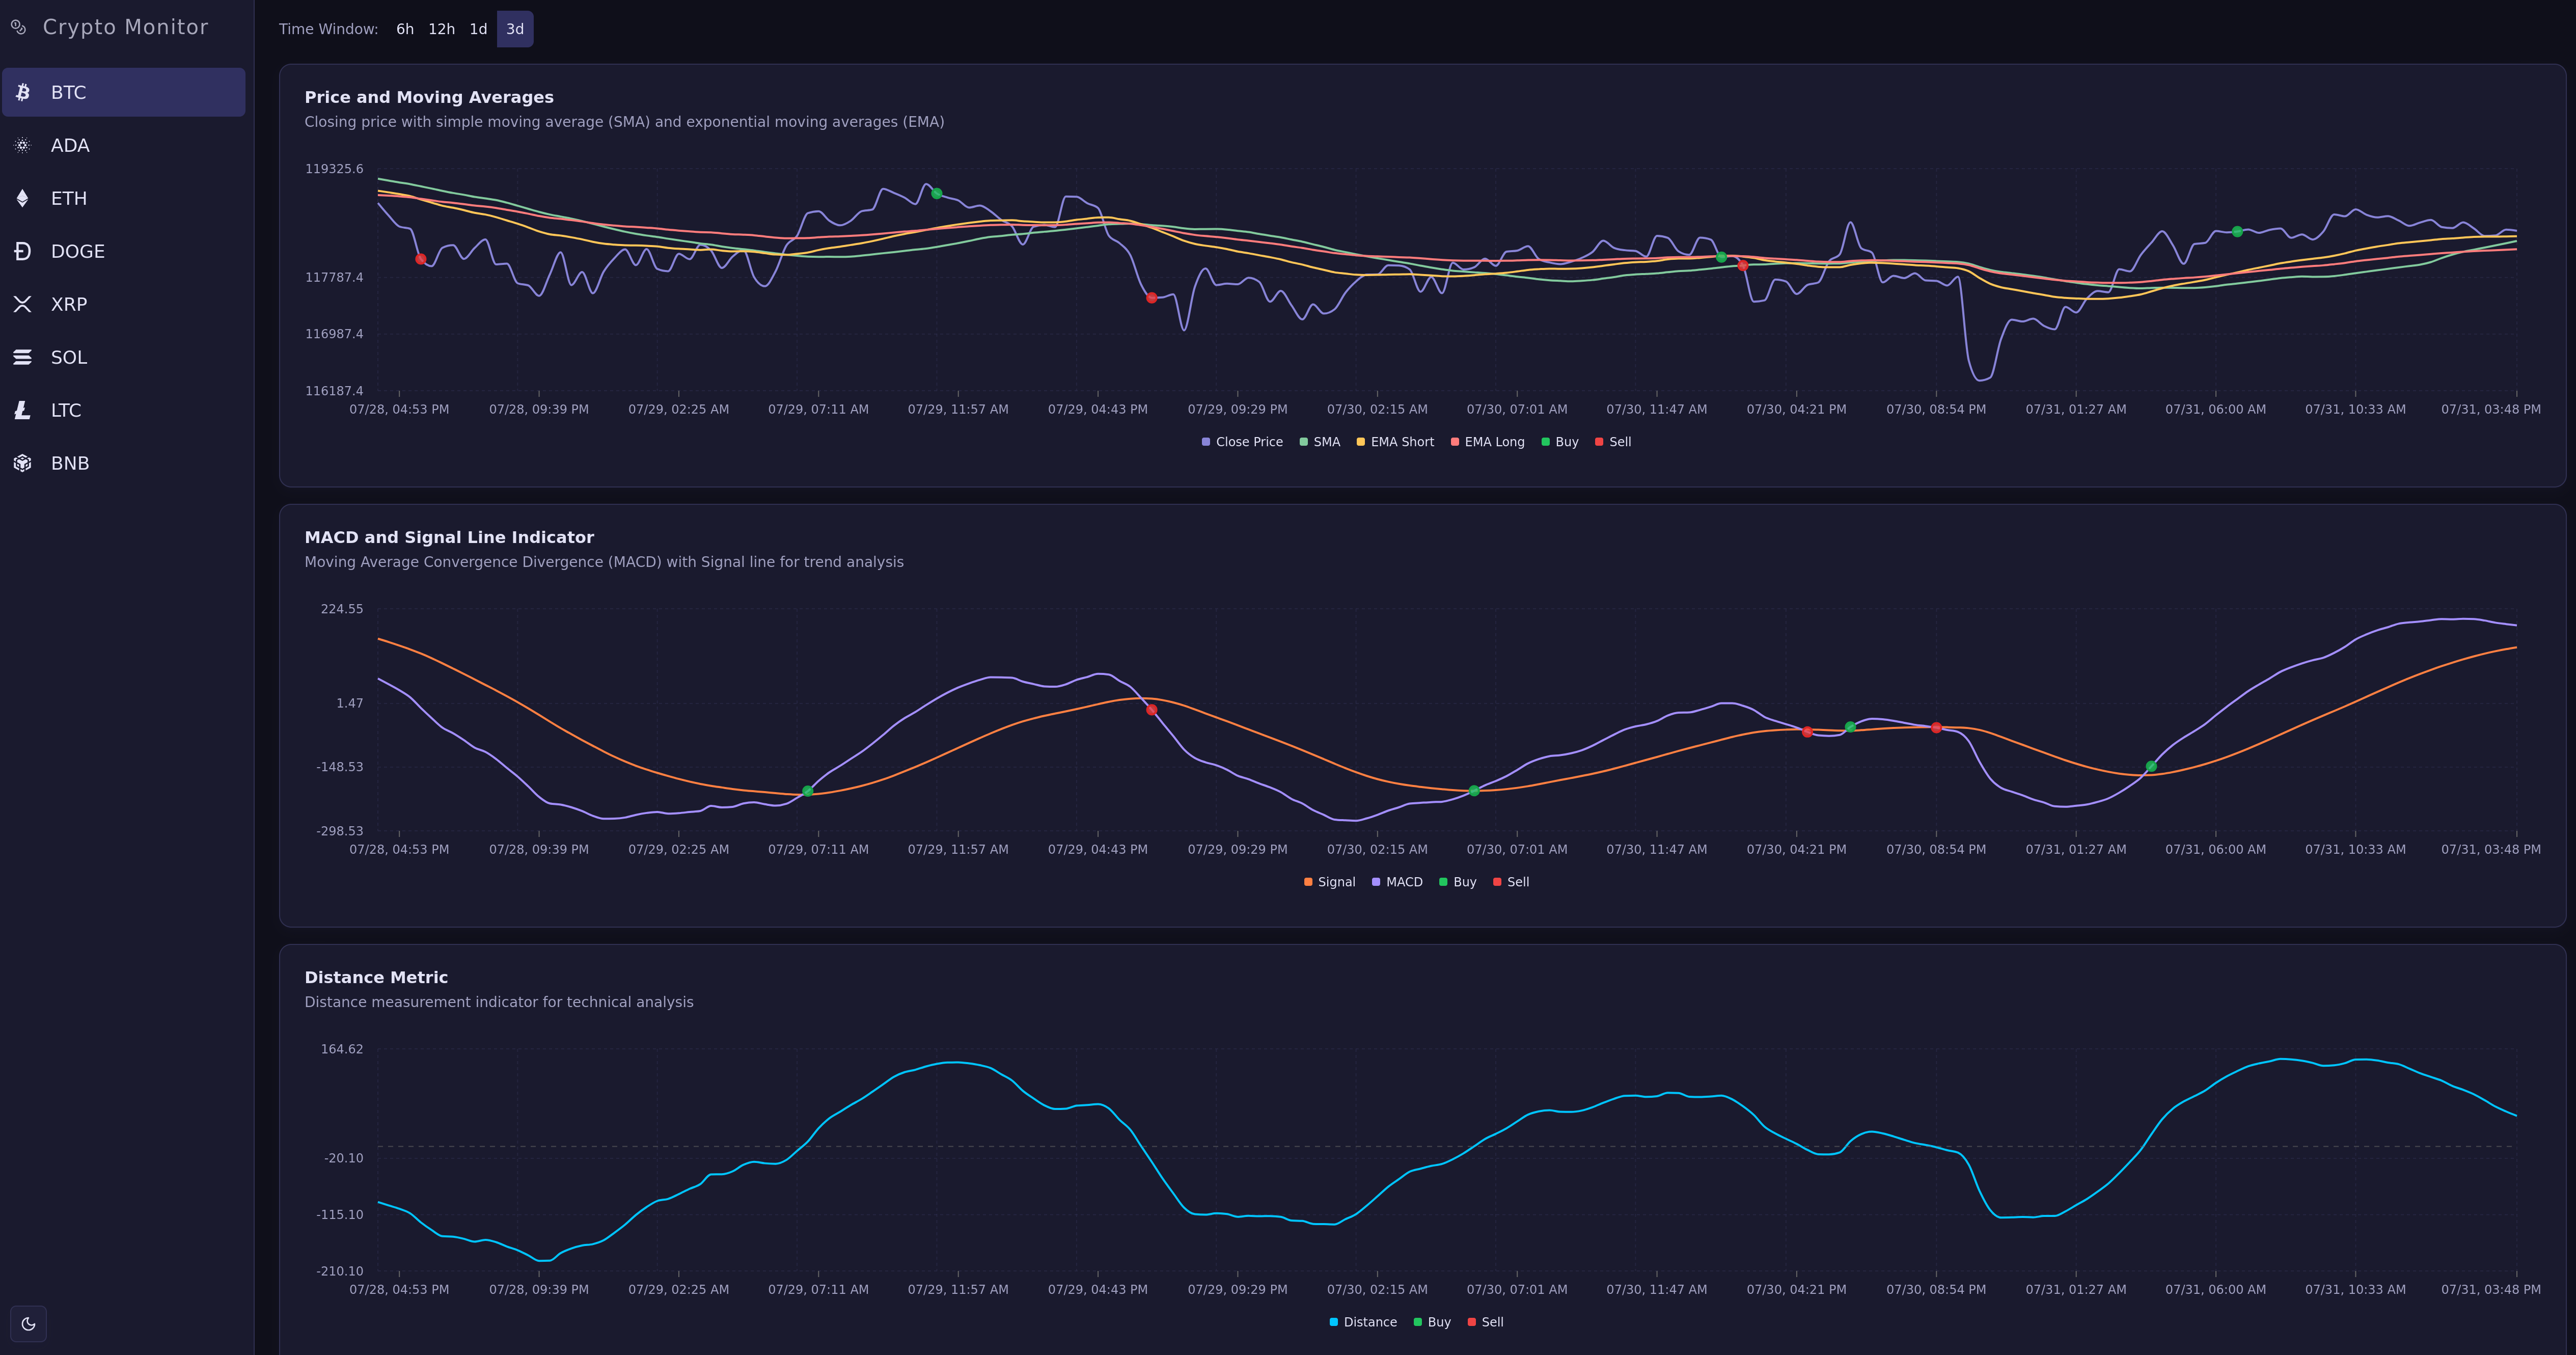
\includegraphics[width=1\textwidth]{UI-full.png}
    \caption{The frontend UI of the Crypto Monitor}
    \label{alg:ui-full}
\end{figure}


\section{Analyzing the predictions}

\subsection{Scenario}
By creating a fake scenario we can make an analysis on the results of the trading strategies.
For the period 28th July - 31st July at 19:00 (3 days total), we will assume that we start with 
\textbf{80k} USD capital, \textbf{10k} for each symbol. 

\begin{itemize}
    \item When there's a signal to \texttt{buy}, we will buy 2k worth of the symbol.
    \item When there is a signal to \texttt{sell}, we will sell all holdings of the symbol (if we have invested any).
\end{itemize}

\subsection{Strategies Recap}
There are 3 strategies in total:
\begin{itemize}
    \item \textbf{EMA Strategy}: Buy/sell based on the EMA crossover.
    \item \textbf{Distance Strategy}: Buy/sell based on the Distance line crossover with $y=0$.
    \item \textbf{Buy \& Hold}: Buy at the start of the 3-day period (80k worth) and sell at the end of it.
\end{itemize}

\subsection{Results}
Table \ref{tab:strategy-performance} shows the overall performance comparison of the three strategies 
over the 3-day period.

\begin{table}[H]
    \centering
    \begin{tabular}{|l|r|r|r|r|r|}
        \hline
        \textbf{Strategy} & \textbf{Final Value} & \textbf{Total Return} & \textbf{Return (\%)} & \textbf{Total Trades} & \textbf{Avg Trades/Symbol} \\
        \hline
        Distance & \$78,963.10 & \$-1,036.90 & -1.30\% & 62 & 7.8 \\
        \hline
        EMA & \$79,535.80 & \$-464.20 & -0.58\% & 21 & 2.6 \\
        \hline
        Buy \& Hold & \$77,638.99 & \$-2,361.01 & -2.95\% & 0 & 0.0 \\
        \hline
    \end{tabular}
    \caption{Overall Strategy Performance Comparison}
    \label{tab:strategy-performance}
\end{table}

Even though we lost money with all strategies, the results show that the 
\textbf{EMA Crossover strategy performed the best} with the smallest loss of -0.58\%, 
followed by the Distance-Based strategy at -1.30\%. The passive Buy \& Hold strategy had the worst 
performance with a -2.95\% loss over the 3-day period.

The per-symbol best-strategy comparison is shown in table \ref{tab:strategy-performance-symbols}.

\begin{table}[H]
    \centering
    \begin{tabular}{|l|l|r|r|r|}
        \hline
        \textbf{Symbol} & \textbf{Better Strategy} & \textbf{Difference} & \textbf{Distance Trades} & \textbf{EMA Trades} \\
        \hline
        BTC-USDT & EMA & \$16.99 & 8 & 5 \\
        \hline
        ADA-USDT & EMA & \$121.92 & 8 & 2 \\
        \hline
        ETH-USDT & Distance & \$3.48 & 8 & 5 \\
        \hline
        DOGE-USDT & EMA & \$102.73 & 8 & 2 \\
        \hline
        XRP-USDT & EMA & \$137.22 & 10 & 1 \\
        \hline
        SOL-USDT & EMA & \$141.79 & 8 & 2 \\
        \hline
        LTC-USDT & Distance & \$13.22 & 6 & 3 \\
        \hline
        BNB-USDT & EMA & \$68.74 & 6 & 1 \\
        \hline
    \end{tabular}
    \caption{Per-symbol Strategy Performance Comparison}
    \label{tab:strategy-performance-symbols}
\end{table}

As we can see, the EMA strategy outperformed the Distance strategy in most symbols, with the exception 
of ETH-USDT and LTC-USDT. This indicates that we should take into account both strategies when making
decisions on when to buy/sell stocks.

\section{Conclusion}
In this project, we successfully implemented an embedded system crypto monitor that can run on a raspberry pi
continuously no matter the internet conditions, with a high efficiency. By utilizing mutexes and condition variables,
we can ensure that the program is fault-tolerant and behaves correctly, as specified by the producer-consumer problem.

The trading strategies we implemented, such as the EMA and Distance strategies, show promising results in predicting 
the market. By utilizing them, we can make better financial decisions. Other strategies that utilize the SMA or
the Pearson correlation can be used, but they might show worse results in high volatile markets like the cryptocurrency market.

\section{Sources}
\begin{itemize}
    \item The web application can be accessed at \url{https://crypto-monitor.nontasbak.com/}
    \item The API for the data can be accessed at \url{https://api-crypto-monitor.nontasbak.com/} (the REST endpoints are \texttt{/sma}, \texttt{/ema}, \texttt{/close}, \texttt{/macd}, \texttt{/signal}, \texttt{/distance})
    \item The source code can be found on the \href{https://github.com/NontasBak/embedded-crypto-monitor}{Github repository}.
\end{itemize}

\begin{thebibliography}{9}

\bibitem{stockprediction}
Ahmet Soydemir.
\textit{Stock Price Prediction with Technical Analysis Tutorial}.
Medium, 2023.
\url{https://medium.com/@ahmettsdmr1312/stock-price-prediction-with-technical-analysis-tutorial-f0ad103cc35f}

\bibitem{exponentialsmoothing}
\textit{Exponential smoothing}.
Wikipedia.
\url{https://en.wikipedia.org/wiki/Exponential_smoothing}

\bibitem{macdstrategy}
\textit{MACD Trading Strategy}.
YouTube.
\url{https://www.youtube.com/watch?v=rf_EQvubKlk}

Thanks to Github Copilot for helping with the final data analysis.

\end{thebibliography}

\end{document}